\section{Esecuzione}

La prima operazione da noi fatta è stata quella di mettere in moto l'impianto da vuoto portando la camera a una pressione di $10^{-3}$ \si{\pascal}, avendo cura di controllare la pressione raggiunta con il vacuometro a catodo freddo.

In seguito abbiamo misurato l'andamento della pressione interna della camera da vuoto in funzione del tempo con la valvola a spillo completamente chiusa. Ciò è stato necessario per misurare la variazione della pressione in camera che, una volta isolata dalla pompa turbomolecolare e dal resto dell'impianto, è dovuta ai soli effetti di degasamento della camera.

Una volta eseguita questa prima serie di misure abbiamo riportato la camera ad una pressione interna di $10^{-3}$ \si{\pascal} per misurare il flusso in entrata a seconda dell'apertura della valvola osservando la seguente procedura:
\begin{itemize}
	\item{portare la camera da vuoto$^1$ ad una pressione di $10^{-3}$ \si{\pascal}, controllando con il vacuometro a catodo freddo di essere ad una pressione minore del fondoscala del vacuometro Pirani}
	\item{spegnere il vacuometro a catodo freddo per evitare l'usura o il deterioramento dello stesso a causa dell'aumento di pressione}
	\item{isolare la camera da vuoto e aprire la valvola a spillo del numero di giri voluto}
	\item{togliere il tappo posto a chiusura della valvola a spillo e misurare, tramite il multimetro e il sistema di acquisizione dati, il variare della pressione interna della camera in funzione del tempo}
	\item{infine riportare la camera da vuoto ad una pressione di $10^{-3}$ \si{\pascal} isolando la pompa turbomolecolare qualora la pressione in camera fosse superiore a qualche Pascal}
\end{itemize}
Mentre la prima serie di misure è stata fatta con la valvola a spillo completamente chiusa, le misure successive hanno invece avuto lo scopo di ottenere i dati di flusso per un'apertura della valvola da 1 a 9 giri completi e di 5.2, 5.4, 5.6 e 5.8 giri.\\

$^1 Nota$: la valvola a spillo presenta al suo interno un volume morto di aria a pressione atmosferica, che se ignorato renderebbe scorretta le misure da noi effettuate. Per ovviare a questo problema abbiamo chiuso la valvola con un tappo e un o-ring in viton e non con la manopola della stessa, in modo tale da rendere il volume morto parte della camera e quindi avere ovunque la stessa pressione misurata dal vacuometro a catodo freddo.

\section{Analisi dati}

Per ogni serie di dati abbiamo ricavato, con il metodo della regressione lineare, un valore della variazione di pressione $\frac{dP}{dt}$. Grazie a questi dati abbiamo poi potuto ottenere una stima del flusso in entrata grazie alla seguente relazione:

\begin{equation}
	Q_{tot} \,\, = \,\, V \frac{dP}{dt}
\end{equation}

Bisogna prestare attenzione che il flusso calcolato ($Q_{tot}$) grazie alla precedente equazione rappresenta il contributo di due differenti fattori: uno è dovuto alla perdita controllata di gas da parte della valvola a spillo ($Q_{valve}$), mentre il secondo è opera degli effetti di degasamento della camera da vuoto e delle altre parti dell'impianto ($Q_{deg}$).

Pertanto, per ricavare Q$_{valve}$ abbiamo dovuto sottrarre al flusso totale calcolato il flusso  dovuto alle perdite intrinseche e virtuali del sistema, ovvero:

\begin{equation}
	Q_{valve} \, = \, Q_{tot} \, - \, Q_{deg}
\end{equation}

I risultati numerici sono esposti nella Tabella \ref{tab:table}

\begin{figure}[h!]
    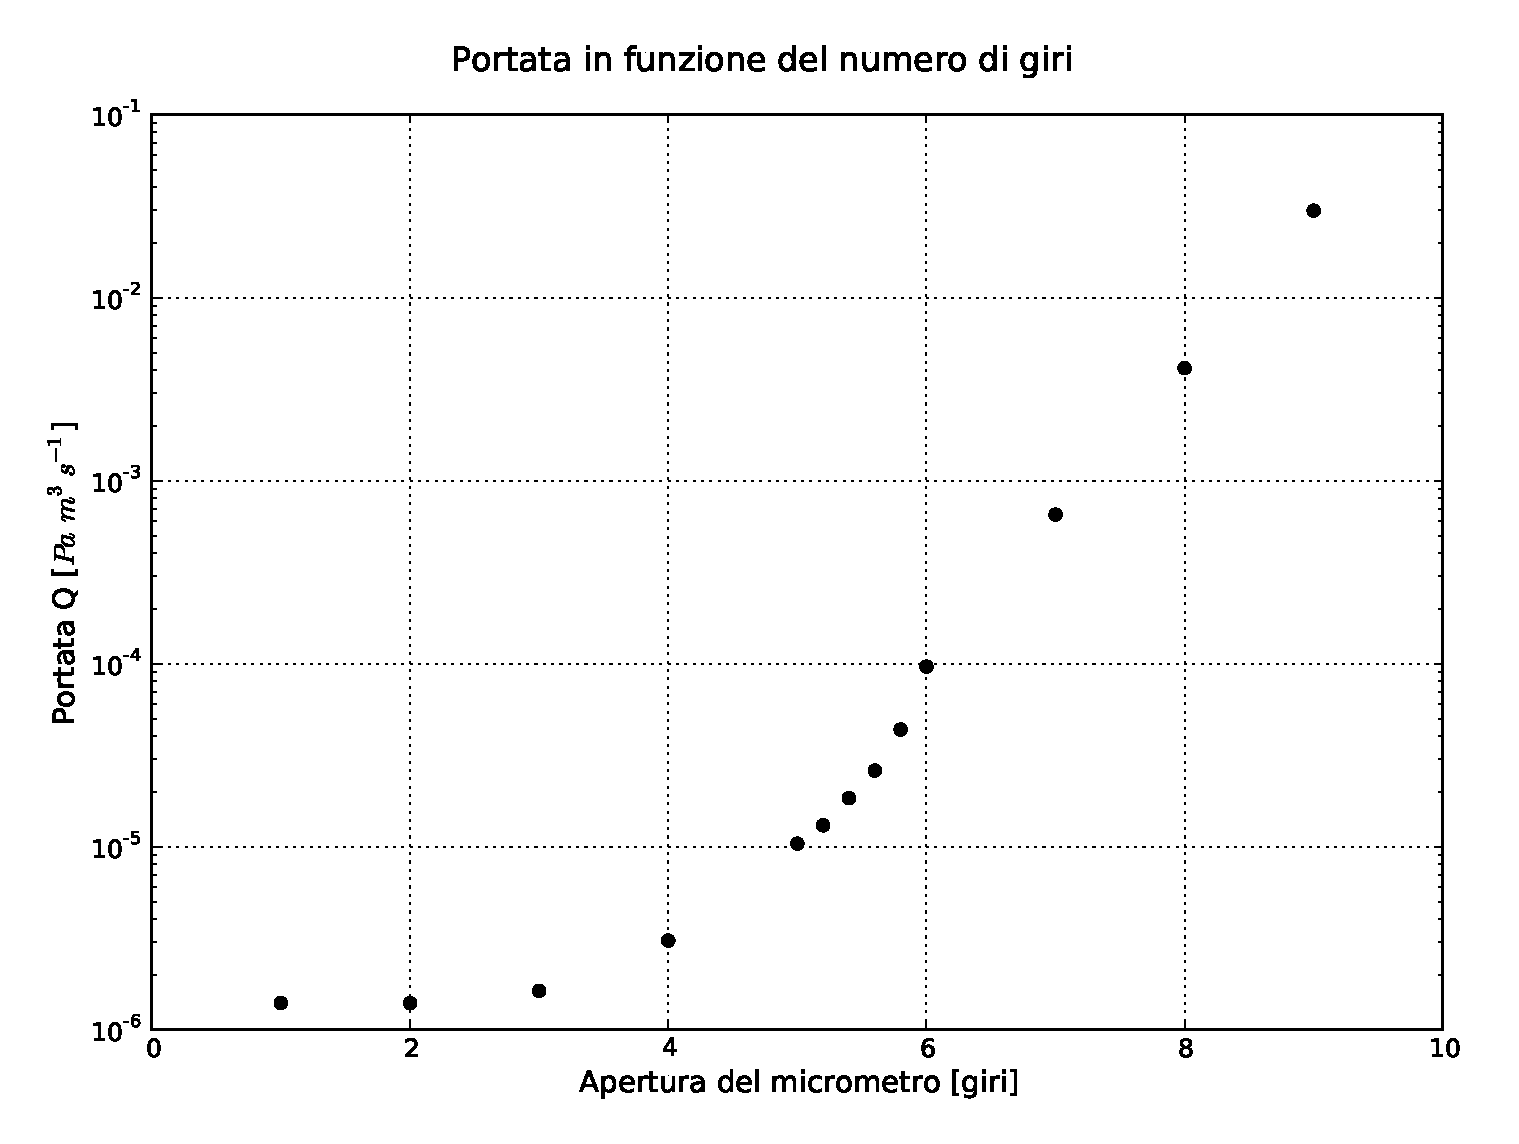
\includegraphics[width=16cm]{graph.pdf}
    \caption{Il grafico mostra i valori elaborati del flusso in entrata a seconda dell'apertura della valvola a spillo. Le barre d'errore non sono
    mostrate in quanto comparabili con la dimensione dei punti sul grafico.}
    \label{fig:graph}
\end{figure}
